\documentclass[]{article}

\usepackage[top=1in, bottom=1.25in, left=0.9in, right=0.9in]{geometry}
\usepackage{titlesec}
\titleformat{\section}
  {\normalfont\Large}
  {\thesection}{1em}{}
\titleformat{\subsection}
  {\normalfont\large}
  {\thesection}{1em}{}
\usepackage{wallpaper}
\ThisURCornerWallPaper{1.0}{img/cover.png}
\usepackage{color}
\usepackage{xcolor}
\usepackage{hyperref}
\definecolor{blue}{rgb}{0.01, 0.28, 1.0}
\definecolor{lightgray}{rgb}{0.95, 0.95, 0.95}
\hypersetup{colorlinks=true, urlcolor=blue, citecolor=blue, filecolor=blue, linkcolor=blue}
\makeatletter
\renewcommand{\maketitle}{\bgroup\setlength{\parindent}{0pt}
\begin{flushleft}
	\vspace{0.5cm}
 	\huge{\@title}\vspace{0.5cm}\\
	\quad\Large Homework (Session 4)\vspace{0.5cm}\\
  	\qquad\large\textit{\@author}
\end{flushleft}\egroup
}
\makeatother
\newcommand{\fakesection}[1]{
	\section*{#1}
	\par\refstepcounter{section}
	\addcontentsline{toc}{section}{#1}
}
\newcommand{\fakesubsection}[1]{
	\subsection*{#1}
	\par\refstepcounter{subsection}
	\addcontentsline{toc}{subsection}{\protect\numberline{\thesubsection}#1}
}
\newcommand{\fakesubsubsection}[1]{
	\subsubsection*{#1}
	\par\refstepcounter{subsubsection}
	\addcontentsline{toc}{subsubsection}{#1}
}
\newcommand{\parx}{\par\noindent}
\usepackage{tikz}
\usepackage{listings}
\usepackage{amssymb}

\usepackage[cachedir=minted]{minted}

%%%%%%%%%%%%%%%%%%%%%%%%%%%%%%%%%%%
%%%%%%%%%%%%%%%%%%%%%%%%%%%%%%%%%%%
%%%%%%%%%%%%%%%%%%%%%%%%%%%%%%%%%%%

\begin{document}

\title{Category Theory for Programmers}
\author{Bruno Vandekerkhove}
\date{}
\maketitle
\vspace{0.5cm}

\tableofcontents

\fakesection{Alternative definition of a natural transformation}

Saunders MacLane defines natural transformations in terms of what's basically a commutative diagram, the naturality square (here with two functors $F$ and $G$, $C\rightarrow D$) : 

\begin{center}
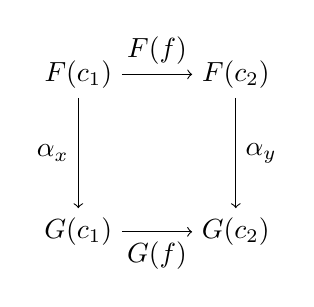
\begin{tikzpicture}
	\node at (-1,1) (1) {$F(c_1)$};
	\node at (1,1) (2) {$F(c_2)$};
	\node at (-1,-1) (3) {$G(c_1)$};
	\node at (1,-1) (4) {$G(c_2)$};
	\draw[->] (1) to node[above]{$F(f)$} (2);
	\draw[->] (1) to node[left]{$\alpha_x$} (3);
	\draw[->] (2) to node[right]{$\alpha_y$} (4);
	\draw[->] (3) to node[below]{$G(f)$} (4);
\end{tikzpicture}
\end{center}

\noindent The rest of this whole paragraph is loosely equivalent with \textit{nLab's} definition of a natural transformation in terms of the cartesian closed monoidal structure \cite{web:ncatlab}. A cartesian monoidal category $C$ is closed when there's an \textit{internal hom} functor $[X,-]:C\rightarrow C$ such that :
$$Hom(a\times b,c)\cong Hom(a,[b,c]=b^c)$$
\noindent Where the rightward map is called currying. The exponential notation is used because the category is cartesian.\\

\par\noindent Since \texttt{Cat} is a cartesian monoidal category the question is if there is an \textit{internal hom} functor $[C,-]:\texttt{Cat} \rightarrow \texttt{Cat} $ which would make it closed such that for $A,C,D\in$ \texttt{Cat} :
$$Funct(A\times C,D)\cong Funct(A,[C,D])$$
\noindent This is true when $[C,D]$ represents the category of functors from $C$ to $D$. The morphisms in that category are natural transformations, and to see what they are we consider a functor $I\rightarrow E$ with $E$ any category and $I$ the  \textit{interval} category (a category with just two objects and one morphism between them, denoted as $\{a\rightarrow b\}$). This functor corresponds to a choice of morphism in $E$. So we can find out what a morphism is in $[C,D]$ by taking a close look at the functors $I\rightarrow[C,D]$. The following holds :
$$Funct(I,[C,D])\cong Funct(I\times C,D)$$
\noindent This means we can consider functors $I\times C\rightarrow D$ instead. The morphisms of the category $I\times C$ are pairs of morphisms in $I$ and $C$ subject to composition laws such that we end up with a commuting diagram :

\begin{center}
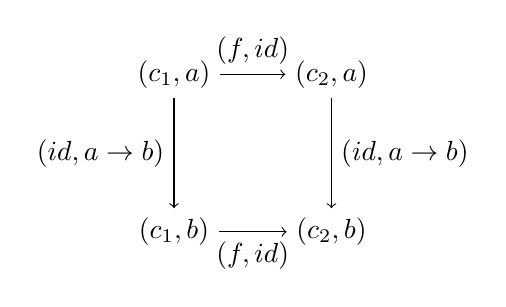
\begin{tikzpicture}
	\node at (-1,1) (1) {$(c_1,a)$};
	\node at (1,1) (2) {$(c_2,a)$};
	\node at (-1,-1) (3) {$(c_1,b)$};
	\node at (1,-1) (4) {$(c_2,b)$};
	\draw[->] (1) to node[above]{$(f,id)$} (2);
	\draw[->] (1) to node[left]{$(id,a\rightarrow b)$} (3);
	\draw[->] (2) to node[right]{$(id,a\rightarrow b)$} (4);
	\draw[->] (3) to node[below]{$(f,id)$} (4);
\end{tikzpicture}
\end{center}

\noindent We can therefor conclude that a natural transformation between functors $C\rightarrow D$ is given by the image of this square in $D$. For a natural transformation $\alpha:F\rightarrow G$ one can trace back the \textit{hom}-isomorphism to end up with a commuting diagram which corresponds to the naturality square depicted at the start of the paragraph (also depicted in Bartosz's book).

% \fakesubsection{}

\fakesection{The bifunctor \texttt{Pair a b}}

Here's an implementation of the \texttt{Pair} bifunctor :

\begin{minted}[xleftmargin=20pt,linenos]{haskell}
import Data.Bifunctor

data Pair a b = Pair a b

instance Bifunctor Pair where
    bimap g h (Pair x y) = Pair (g x) (h y)
    first g (Pair x y) = Pair (g x) y
    second h (Pair x y) = Pair x (h y)
\end{minted}

\noindent\texttt{Pair a b} can be proven to be a bifunctor with equational reasoning (it's enough to show that it is functorial in each argument separately) :

\begin{minted}[xleftmargin=20pt,linenos]{haskell}
bimap id id (Pair x y) = Pair (id x) (id y)
	= Pair x y
	= id (Pair x y)
bimap (f . g) id (Pair x y) = Pair (f . g x) (id y)
	= Pair (f . g x) y
	= bimap g . (Pair (f x) y)
	= bimap g . bimap f (Pair x y)
-- bimap id (f . g) (Pair x y) boils down to the same thing
\end{minted}

\noindent This is not a surprise given that \texttt{Pair} is isomorphic with the \texttt{(,)} bifunctor. We now show that the above implementation is equivalent to using the default ones :

\begin{minted}[xleftmargin=20pt,linenos]{haskell}
bimap g h (Pair x y) = first g . second h = first g . (Pair x (h y)) = Pair (g x) (h y)
first g = bimap g id = Pair (g x) (id y) = Pair (g x) y
second h = bimap id h = Pair (id x) (h y) = Pair x (h y)
\end{minted}

\fakesection{Isomorphism of \texttt{Maybe} and \texttt{Maybe'}}

\noindent It can be shown that \texttt{Maybe'} and \texttt{Maybe} are isomorphic by constructing two mappings and using equality reasoning to show that they're each other's inverse :

\begin{minted}[xleftmargin=20pt,linenos]{haskell}
import Data.Functor.Identity
import Data.Functor.Const

type Maybe' a = Either (Const () a) (Identity a)

toMaybe' :: Maybe a -> Maybe' a
toMaybe' Nothing = Left (Const ())
toMaybe' (Just a) = Right (Identity a)

toMaybe :: Maybe' a -> Maybe a
toMaybe (Left (Const ())) = Nothing
toMaybe (Right (Identity a)) = Just a

toMaybe' . toMaybe (Left (Const ())) = toMaybe' Nothing = Left (Const ())
toMaybe' . toMaybe (Right (Identity a)) = toMaybe' (Just a) = Right (Identity a)

toMaybe . toMaybe' Nothing = toMaybe (Left (Const ())) = Nothing
toMaybe . toMaybe' (Just a) = toMaybe (Right (Identity a)) = Just a
\end{minted}

\fakesection{The \texttt{PreList} bifunctor}

The \texttt{PreList} bifunctor can be implemented as follows :

\begin{minted}[xleftmargin=20pt,linenos]{haskell}
data PreList a b = Nil | Cons a b

instance BiFunctor (PreList a b) where
	bimap g h Nil = Nil
	bimap g h (Cons a b) = Cons (g a) (h b)
\end{minted}

\noindent Aside from proving that it is functorial in both arguments (which is analogous to what we did for \texttt{Pair}) it can be noted that it is equivalent to \texttt{Either (Const () a) (a,b)} which is a bifunctor because \texttt{Either} and \texttt{(,)} are bifunctors and \texttt{Const ()} is a functor. The reasoning is similar to what happens with \texttt{Maybe = Either (Const () a) (Identity a)} except that in that case you really end up with a functor because the type parameter is the same for both parts of the sum.

\fakesection{\texttt{K2}, \texttt{Fst} and \texttt{Snd}}

Implementation of \texttt{bimap} follows :

\begin{minted}[xleftmargin=20pt,linenos]{haskell}
instance BiFunctor (K2 c a b) where
	bimap _ _ = id
instance BiFunctor (Fst a b) where
	bimap g _ (Fst a) = Fst (g a)
instance BiFunctor (Snd a b) where
	bimap _ h (Snd b) = Fst (h b)
\end{minted}

\noindent In the referenced study \texttt{K2} is described as the bifunctorial `cousin' of \texttt{K1} which is a constant. They're part of a repertoire of components called \textit{`polynomial (bi)functors'} which are used by the author to deal with data types in a generic way.

%\fakesection{The functoriality of \texttt{std::map}}
%
%It looks like we're dealing with $a\rightarrow \texttt{Maybe}\ b$ given the data structure's implementation of \texttt{find} :
%\begin{quote}
%Iterator to an element with key equivalent to key. If no such element is found, past-the-end (see end()) iterator is returned.
%\end{quote}


\fakesection{Natural transformation of \texttt{Maybe} to \texttt{List}}

Here's a natural transformation from \texttt{Maybe} to \texttt{List} and a proof that it satisfies the naturality condition :

\begin{minted}[xleftmargin=20pt,linenos]{haskell}
alpha :: Maybe a -> [a]
alpha Nothing = []
alpha (Just x) = [x]

fmap f (alpha Nothing) = fmap f [] = []
alpha (fmap f Nothing) = alpha Nothing = []

fmap f (alpha (Just x)) = fmap f [x] = [f x]
alpha (fmap f (Just x)) = alpha (Just (f x)) = [f x]
\end{minted}

\noindent Many more are possible, which is illustrated in the next challenge. It can be noted that Haskell's parametric polymorphism made the proof unnecessary, which was hinted at in the previous lesson where the `magic trick' showed that polymorphic functions do nothing to the elements themselves so the order of application isn't important.

\fakesection{Natural transformation from \texttt{Reader} to \texttt{List} or \texttt{Maybe}}

There's an infinite amount of natural transformations from \texttt{Reader ()} to \texttt{List} because you can transform to the empty list or to a series of applications of $g$ to $()$ :

\begin{minted}[xleftmargin=20pt,linenos]{haskell}
-- :: Reader () a -> [a]
alpha0 (Reader g) = []
alpha1 (Reader g) = [g ()]
alpha2 (Reader g) = [g (), g ()]
...
\end{minted}

\noindent This doesn't hold in the case of \texttt{Reader Bool} and \texttt{Maybe} where you can only transform in three ways (returning \texttt{Nothing}, \texttt{Just (g True)} and \texttt{Just (g False)} respectively).

%\fakesection{Naturality condition holds}
%
%Diagram chasing means that you take a commuting diagram and go through it to construct a syllogism. In this case we want to prove that the horizontal composition retains naturality. The diagram the following is based on is displayed on page 177 of the book :
%
%\begin{figure}[h]
%\centering
%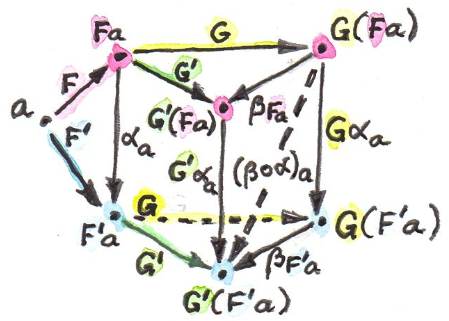
\includegraphics[width=0.5\textwidth]{img/diagram.png}
%\end{figure}

\bibliographystyle{plain}
\bibliography{References}
\addcontentsline{toc}{section}{References}

\end{document}